%% LyX 2.3.6 created this file.  For more info, see http://www.lyx.org/.
%% Do not edit unless you really know what you are doing.
\documentclass[english]{article}
\usepackage[T1]{fontenc}
\usepackage[latin9]{inputenc}
\usepackage[active]{srcltx}
\usepackage{float}
\usepackage{textcomp}
\usepackage{url}
\usepackage{amsmath}
\usepackage{graphicx}

\makeatletter

%%%%%%%%%%%%%%%%%%%%%%%%%%%%%% LyX specific LaTeX commands.
%% Because html converters don't know tabularnewline
\providecommand{\tabularnewline}{\\}
\floatstyle{ruled}
\newfloat{algorithm}{tbp}{loa}
\providecommand{\algorithmname}{Algorithm}
\floatname{algorithm}{\protect\algorithmname}

%%%%%%%%%%%%%%%%%%%%%%%%%%%%%% Textclass specific LaTeX commands.
\newenvironment{lyxcode}
	{\par\begin{list}{}{
		\setlength{\rightmargin}{\leftmargin}
		\setlength{\listparindent}{0pt}% needed for AMS classes
		\raggedright
		\setlength{\itemsep}{0pt}
		\setlength{\parsep}{0pt}
		\normalfont\ttfamily}%
	 \item[]}
	{\end{list}}

\makeatother

\usepackage{babel}
\begin{document}
\title{Constructing features using a hybrid genetic algorithm}
\author{Ioannis G. Tsoulos\thanks{Corresponding author. Email: itsoulos@uoi.gr}}
\date{Department of Informatics and Telecommunications, University of Ioannina,
Greece}
\maketitle
\begin{abstract}
A hybrid procedure that incorporates Grammatical Evolution and a weight
decaying technique is proposed here for various problems, classification
or regression. The proposed method has two main phases: the creation
of features and the evaluation of these features. During the first
phase, using Grammatical Evolution, new features are created as non-linear
combinations of the original features of the datasets. In the second
phase, based on the characteristics of the first phase, the original
data set is modified and a neural network trained with a genetic algorithm
is applied to this dataset. The proposed method was applied to an
extremely wide set of datasets from the relevant literature and the
experimental results were compared with 4 other techniques. 
\end{abstract}
\textbf{Keywords}: Genetic algorithm, machine learning, neural networks,
Grammatical Evolution.

\section{Introduction}

Artificial Neural networks (ANNs) are programming tools \cite{nn1,nn2},
based on a series of parameters that commonly called weights or processing
units. They have been used in a variety of problems from different
scientific areas such as physics \cite{nnphysics1,nnphysics2,nnphysics3},
chemistry \cite{nnchem1,nnchem2,nnchem3}, economics \cite{nnecon1,nnecon2,nncecon3},
medicine \cite{nnmed1,nnmed2} etc. A common way to express a neural
network is a function $N(\overrightarrow{x},\overrightarrow{w})$,
with $\overrightarrow{x}$ the input vector (commonly called pattern)
and $\overrightarrow{w}$ the weight vector. A method that trains
a neural network should be used to estimate the vector $\overrightarrow{w}$
for the certain problem. The training procedure can be formulated
also an optimization problem, where the target is to minimize the
so called error function:
\begin{equation}
E\left(N\left(\overrightarrow{x},\overrightarrow{w}\right)\right)=\sum_{i=1}^{M}\left(N\left(\overrightarrow{x}_{i},\overrightarrow{w}\right)-y_{i}\right)^{2}\label{eq:eq1}
\end{equation}
In equation \ref{eq:eq1} the set $\left(\overrightarrow{x_{i}},y_{i}\right),\ i=1,...,M$
is the dataset used to train the neural network, with $y_{i}$ being
the actual output for the point $\overrightarrow{x_{i}}$ . The neural
network $N(\overrightarrow{x},\overrightarrow{w})$ can be modeled
as a summation of processing units as proposed in \cite{nnc}:
\begin{equation}
N\left(\overrightarrow{x},\overrightarrow{w}\right)=\sum_{i=1}^{H}w_{(d+2)i-(d+1)}\sigma\left(\sum_{j=1}^{d}x_{j}w_{(d+2)i-(d+1)+j}+w_{(d+2)i}\right)\label{eq:nn}
\end{equation}
where $H$ is the number of processing units of the neural network
and $d$ is the dimension of vector $\overrightarrow{x}$. The function
$\sigma(x)$ is the sigmoid function defined as: 
\begin{equation}
\sigma(x)=\frac{1}{1+\exp(-x)}\label{eq:sig}
\end{equation}
From the equation \ref{eq:nn} one can obtain that the dimension of
weight vector $w$ is computed as: $w=(d+2)H$. The function of equation
\ref{eq:eq1} has been minimized with a variety of optimization methods
during the past years such as: the Back Propagation method \cite{bpnn,bpnn2},
the RPROP method \cite{rpropnn,rpropnn3,rpropnn2}, Quasi Newton methods
\cite{quasinn,quasinn2}, Particle Swarm Optimization \cite{psonn,psonn2}
etc. All the previously mentioned methods have to overcome two major
problems:
\begin{itemize}
\item Excessive computational times, because they require processing time
proportional to the dimension of the objective problem and the number
of processing units as well. For example, a neural network of $H=10$
processing units applied to a test data with $d=3$, is considered
as an optimization problem with dimension $w=(d+2)H=50$. An extensive
discussion on the problems occurred by the dimensionality on neural
networks is presented in \cite{nndimension}. A common approach to
overcome this problem is to use the PCA technique to reduce the dimensionality
of the objective problem \cite{nnpca1,nnpca2,nnpca3} i.e. the parameter
$d$.
\item The ovetfitting problem. It is quite common for these methods to produce
poor results, when they are applied to data (test data) not previously
used in the training procedure. This problem is discussed in detail
in the article of Geman et all \cite{nngeman} as well as in the article
of Hawkins \cite{nnhawkins}. A variety of methods have been proposed
to overcome this problem such as are weight sharing \cite{nnsharing1},
pruning \cite{nnprunning1,nnprunning2,nnprunning3}, the dropout technique
\cite{nndrop1}, early stopping \cite{nnearly1,nnearly2}, and weight
decaying \cite{nndecay1,nndecay2}. 
\end{itemize}
This article proposes a method that tackle both the above problems
using two major steps. During the first step a new set of features
is created from the initial features using a procedure based on the
Grammatical Evolution technique \cite{ge1}. A feature is a measurement
that defines a property of the objective problem and the series of
all measurements forms a pattern. A feature can be a integer value,
a double precision value or even a string literature. In our case
we consider only numeric values for the features. The number of features
of each pattern is the dimensionality of the problem defined as $d$
in this work. The procedure of Feature Construction with Grammatical
Evolution was introduced in the work of Gavrilis et al \cite{fc1}
and it has been used with success in Spam Identification\textbf{ }\cite{fc2}\textbf{,
}Fetal heart classification\textbf{ }\cite{fc3}\textbf{, }epileptic
oscillations in clinical intracranial electroencephalograms \cite{fc4}
etc. The outcomes of the first phase are the modified training and
testing data according to the created features. During the second
step, a genetic algorithm that incorporates a weight decaying procedure
is used to train a neural network on the modified data of the first
step.

Genetic algorithms are methods based on biological observations such
as reproduction and mutation \cite{genetic1,genetic2}. The genetic
algorithms work by creating and maintaining o population of candidate
solutions (chromosomes). This population is altered iteratively though
operations such as crossover and mutation until some stopping criteria
are met. They have many advantages such as simplicity in the implementation,
endurance in noise, they can be easily palellelized etc. Also, the
have been applied in many problems such as aerodynamic optimization
\cite{par1}, steel structure optimization \cite{par2}, brain images
\cite{par3} etc. They have been used to train neural networks in
various research papers such as the work of Leung et al \cite{geneticnn1}
which estimates the structure and the weights of a neural network
through a genetic algorithm, the evolution of a neural networks for
daily rainfall--runoff forecasting \cite{geneticnn2}, evolution
of neural networks to predict the deformation modulus of rock masses
\cite{geneticnn3} etc. 

The idea of feature construction has been examined by various researched
in the relevant literature such as the work of Smith and Bull \cite{genfc1},
who used a tree genetic programming approach to construct features
from the original ones. Another approach to construct features using
genetic programming was proposed by Neshatian et al \cite{genfc2},
where the genetic programming utilized an entropy based fitness function
that maximizes the purity of class intervals. Another evolutionary
approach was proposed by Li and Yin for feature selection using gene
expression data \cite{genfc3}. Lastly, a recent work that utilizes
a genetic programming approach and the information gain ratio (IGR)
was proposed by Ma and Teng\cite{genfc4} to construct features from
the original ones.

In the problems of classification and regression, as the number of
features increases additional examples are needed in order to achieve
good results in training a model but also to maintain good generalization
skills in unknown data. Of course, adding new examples to the training
process is almost never possible and this results in poor performance
in the control data. For this reason the original data set must be
transformed into a new one, which gives better generalization skills
to the learning models. According to the Cover's theorem\cite{cover},
there is at least one non-linear extension of the original feature
vector, so that with this extension a linear separation of the set
of patterns can be made. Many techniques have been proposed in this
direction that try to detect such nonlinear extensions. The proposed
method uses a hybrid approach, in which first new features are constructed
using Grammatical Evolution and then these features are evaluated
by a neural network that appropriately trains a genetic algorithm.
In the first phase the creation of new features is done in such a
way as to achieve the best possible learning accuracy. The methods
that can be used to convert attributes are grouped into three categories:
feature selection, feature construction, and feature reduction. The
second case is the most difficult, as it does not simply require reducing
the size of the problem but also the non-linear creation of new features
from the old ones. 

The proposed technique can overcome other techniques from the modern
literature, as it does not require prior knowledge of the objective
problem, it can be applied with the exact same procedure to both categorization
problems and function learning problems. In addition it can be used
to discover hidden function dependencies between the original features
of the problem and because it is based on Grammatical Evolution, the
user can add and subtract functions or even allow the algorithm to
construct new functions to better learn the data set. Still, the final
characteristics of the method can be evaluated by any computational
intelligence model without any additional processing. In the present
method, these characteristics are evaluated by an artificial neural
network, but something that could change. 

The rest of this paper is organized as follows: in section \ref{sec:Method-description}
the proposed method is described in detail, in section \ref{sec:Experiments}
the proposed method is tested on a series of well know datasets from
the relevant literature and the results are compared to those of a
simple genetic algorithm and finally in section \ref{sec:Conclusions}
some conclusions are presented.

\section{Method description\label{sec:Method-description}}

The proposed method has two major phases. In the a procedure that
exploits the Grammatical Evolution technique is used, in order to
create new features from the old ones. The new features are evaluated
using a Radial Basis Function (RBF) \cite{rbf1} neural network with
$H$ hidden nodes. The RBF network is used during this phase instead
of a neural network because the training procedure for RBF networks
are must faster than these of neural networks. In the second phase,
a hybrid genetic algorithm trains a neural network using the constructed
features of the first phase. 

\subsection{The usage of Grammatical Evolution\label{subsec:Transformation-procedure}}

Grammatical evolution is a evolutionary procedure, where the chromosomes
are represent production rules from a BNF (Backus--Naur form) grammar\cite{bnf1},
which is used very often to describe the syntax of programming languages,
documents formats etc. These grammars are defined as the set \textbf{$G=\left(N,T,S,P\right)$},
where
\begin{itemize}
\item \textbf{$N$ }is the set of non terminal symbols, which produce through
production rules series of terminal symbols.
\item \textbf{$T$ }is the set of terminal symbols.\textbf{ }
\item $S$ is a non terminal symbol called also start symbol
\item \textbf{$P$ }is a set of production rules in the form \textbf{$A\rightarrow a$
}or\textbf{ $A\rightarrow aB,\ A,B\in N,\ a\in T$.}
\end{itemize}
The production procedure initiates from the start symbol of the BNF
grammar and iteratively produces programs by replacing non terminal
symbols with the right hand of the production rules that will be selected
according to the value of each element in the chromosome\textbf{.}
In the proposed method the BNF grammar of the Figure \ref{fig:BNF-grammar-of}
was used to create a new feature from the initial features. The symbols
that are in <> are considered as non terminal symbols. The parameter
N denotes the number of original features. Typically a chromosome
$x$ in the grammatical evolution is expressed as series of binary
values 0 or 1. In the current work in order to simplify the mapping
procedure and to increase the speed of the algorithm every element
of each chromosome is considered as an integer in a predefined range.
For our case the range $[0,255]$ was used but of course this could
be easily changed.

Take for example the chromosome $x=\left[9,8,6,4,16,10,17,23,8,14\right]$
and $N=3$. The valid expression\textbf{ $f(x)=x_{2}+\cos\left(x_{3}\right)$
}is created using a series of production steps shown in Table \ref{tab:table_with_steps}.
An expression is considered as valid if contains only terminal symbols.\textbf{
}Each number in\textbf{ }the parentheses stands for the sequence number
of the production rule. Hence, the process to produce $N_{f}$ features
from the original  have as follows:
\begin{enumerate}
\item Every chromosome $Z$ is split into $N_{f}$ parts. Each part $g_{i}$
will be used to construct a feature.
\item For every part $g_{i}$ construct a feature $t_{i}$ using the grammar
given in Figure \ref{fig:BNF-grammar-of}
\item Create a mapping function 
\begin{equation}
G(\overrightarrow{x},Z)=\left(t_{1}\left(\overrightarrow{x},Z\right),t_{2}\left(\overrightarrow{x},Z\right),\ldots,t_{N_{f}}\left(\overrightarrow{x},Z\right)\right)\label{eq:mapping}
\end{equation}
where $\overrightarrow{x}$ is a pattern from the original set and
$Z$ is the chromosome.
\end{enumerate}
\begin{figure}
\caption{BNF grammar of the proposed method.\label{fig:BNF-grammar-of}}

\begin{lyxcode}
S::=<expr>~~~(0)~

<expr>~::=~~(<expr>~<op>~<expr>)~~(0)~~~~~~~~~~~~~

~~~~~~~~~~~|~<func>~(~<expr>~)~~~~(1)~~~~~~~~~~~~~

~~~~~~~~~~~|<terminal>~~~~~~~~~~~~(2)~

<op>~::=~~~~~+~~~~~~(0)~~~~~~~~~~~~~

~~~~~~~~~~~|~-~~~~~~(1)~~~~~~~~~~~~~

~~~~~~~~~~~|~{*}~~~~~~(2)~~~~~~~~~~~~~

~~~~~~~~~~~|~/~~~~~~(3)

<func>~::=~~~sin~~(0)~~~~~~~~~~~~~

~~~~~~~~~~~|~cos~~(1)~~~~~~~~~~~~~

~~~~~~~~~~~|exp~~~(2)~~~~~~~~~~~~~

~~~~~~~~~~~|log~~~(3)

<terminal>::=<xlist>~~~~~~~~~~~~~~~~(0)~~~~~~~~~~~~~~~~~~~~~~

~~~~~~~~~~~|<digitlist>.<digitlist>~(1)

<xlist>::=x1~~~~(0)~~~~~~~~~~~~~~

~~~~~~~~~~~|~x2~(1)~~~~~~~~~~~~~~

~~~~~~~~~~~\dots \dots \dots{}~~~~~~~~~~~~~

~~~~~~~~~~~|~xN~(N)

<digitlist>::=<digit>~~~~~~~~~~~~~~~~~~(0)~~~~~~~~~~~~~~~~~

~~~~~~~~~~~|~<digit><digit>~~~~~~~~~~~~(1)

~~~~~~~~~~~|~<digit><digit><digit>~~~~~(2)

<digit>~~::=~0~(0)~~~~~~~~~~~~~

~~~~~~~~~~~|~1~(1)~~~~~~~~~~~~~

~~~~~~~~~~~|~2~(2)~~~~~~~~~~~~~

~~~~~~~~~~~|~3~(3)~~~~~~~~~~~~~

~~~~~~~~~~~|~4~(4)~~~~~~~~~~~~~

~~~~~~~~~~~|~5~(5)~~~~~~~~~~~~~

~~~~~~~~~~~|~6~(6)~~~~~~~~~~~~~

~~~~~~~~~~~|~7~(7)~~~~~~~~~~~~~

~~~~~~~~~~~|~8~(8)~~~~~~~~~~~~~

~~~~~~~~~~~|~9~(9)
\end{lyxcode}
\end{figure}
\begin{table}
\caption{Steps to produce a valid expression from the BNF grammar.\label{tab:table_with_steps}}

\begin{tabular}{|c|c|c|}
\hline 
String & Chromosome & Operation\tabularnewline
\hline 
\hline 
<expr> & 9,8,6,4,16,10,17,23,8,14 & $9\mod3=0$\tabularnewline
\hline 
(<expr><op><expr>) & 8,6,4,16,10,17,23,8,14 & $8\mod3=2$\tabularnewline
\hline 
(<terminal><op><expr>) & 6,4,16,10,17,23,8,14 & $6\mod2=0$\tabularnewline
\hline 
(<xlist><op><expr>) & 4,16,10,17,23,8,14 & $4\mod3=1$\tabularnewline
\hline 
(x2<op><expr>) & 16,10,17,23,8,14 & $16\mod4=0$\tabularnewline
\hline 
(x2+<expr>) & 10,17,23,8,14 & $10\mod3=1$\tabularnewline
\hline 
(x2+<func>(<expr>)) & 17,23,8,14 & $17\mod4=1$\tabularnewline
\hline 
(x2+cos(<expr>)) & 23,8,14 & $23\mod2=1$\tabularnewline
\hline 
(x2+cos(<terminal>)) & 8,14 & $8\mod2=0$\tabularnewline
\hline 
(x2+cos(<xlist>)) & 14 & $14\mod3=2$\tabularnewline
\hline 
(x2+cos(x3)) &  & \tabularnewline
\hline 
\end{tabular}
\end{table}


\subsection{Feature construction \label{subsec:Feature-construction}}

The steps of the algorithm for the first phase are:
\begin{enumerate}
\item \textbf{Initialization step}

\begin{enumerate}
\item \textbf{Set} iter=0, generation number.
\item \textbf{Construct} the set $\mbox{TR}=\left\{ \left(\overrightarrow{x_{1}},y_{1}\right),\left(\overrightarrow{x_{2}},y_{2}\right),\ldots,\left(\overrightarrow{x_{M}},y_{M}\right)\right\} $,
which is the original train set.
\item \textbf{Set} $N_{c}$ the number of chromosomes\textbf{ }and $N_{f}$
the number of desired constructed features. These options are defined
by the user. 
\item \textbf{Initialize} randomly in range $[0,255]$ the integer chromosomes
$Z_{i},i=1\ldots N_{c}$ 
\item \textbf{Set} $N_{g}$ as the maximum number of generations allowed.
\item \textbf{Set} $p_{s}\in[0,1]$ as the selection rate and $p_{m}\in[0,1]$
the mutation rate.
\end{enumerate}
\item \textbf{Termination check.} \textbf{If} iter>=$N_{g}$ \textbf{goto}
step \ref{enu:Obtain-the-best}. \label{enu:Termination-check.-If}
\item \textbf{Estimate} the fitness $f_{i}$ of every chromosome $Z_{i}$
with the following procedure:\label{enu:Calculate-the-corresponding}

\begin{enumerate}
\item \textbf{Use} the procedure described in subsection \ref{subsec:Transformation-procedure}
and create $N_{f}$ features.
\item \textbf{Create} a modified training set 
\begin{equation}
\mbox{TN}=\left\{ \left(G\left(\overrightarrow{x_{1}},Z_{i}\right),y_{1}\right),\left(G\left(\overrightarrow{x_{2}},Z_{i}\right),y_{2}\right),\ldots,\left(G\left(\overrightarrow{x_{M}},Z_{i}\right),y_{M}\right)\right\} 
\end{equation}
 
\item \textbf{Train} an RBF neural network $C$ with $H$ processing units
on the modified training set $\mbox{TN }$using the following train
error
\begin{equation}
f_{i}=\sum_{j=1}^{M}\left(C\left(G\left(\overrightarrow{x_{j}},Z_{i}\right)\right)-y_{j}\right)^{2}
\end{equation}
\end{enumerate}
\item \textbf{Genetic Operators}

\begin{enumerate}
\item \textbf{Selection procedure: }Initially the  chromosomes\textbf{ }are
sorted according to their fitness value.\textbf{ }The best chromosomes
are placed in the beginning of the population and the worst at the
end.\textbf{ }The best $\left(1-p_{s}\right)\times N_{c}$ chromosomes
are transferred to the next generation intact.\textbf{ }The remain
chromosomes\textbf{ }are substituted by offsprings created through
the crossover and mutation procedures.
\item \textbf{Crossover procedure: }In this process for every produced offspring
two mating chromosomes (parents) are selected from the previous population
using tournament selection. The\textbf{ }tournament selection is a
rather simple selection mechanism defined as:\textbf{ }First a set
of $K>1$ randomly selected chromosomes is constructed and subsequently
the chromosome with the best fitness value in the previous set is
selected as mating chromosome. Having selected the two parents for
the offrpsing, the offspring is formed using the one point crossover.
In one - point crossover a random point is selected for the two parents
and their right-hand side subchromosomes are exchanged.
\item \textbf{Mutation procedure: }For every element of each chromosome
a random number $r\in\left[0,1\right]$ is taken. If $r\le p_{m}$
then this element is altered randomly by producing a new integer number.
\end{enumerate}
\item \textbf{Set} iter=iter+1 and \textbf{goto} Step \ref{enu:Termination-check.-If}.
\item \textbf{Get }the best chromosome in the population defined as $Z_{l}$
with the corresponding fitness value $f_{l}$\textbf{ }and \textbf{Terminate}.\textbf{\label{enu:Obtain-the-best}}
\end{enumerate}

\subsection{Weight decay mechanism}

The quantity $x$ in the equation \ref{eq:sig} of the sigmoid function
is calculated through many calculations involving the input patterns
as well as the weight vector. If the value within the function is
too large, then the sigmoid function tends to 0 and this will result
in the neural network losing what generalization possibilities it
has. In order to estimate the effect of this issue, the quantity\textbf{
$B\left(N\left(\overrightarrow{x},\overrightarrow{w}\right),F\right)$
}is defined\textbf{ }as shown in the Algorithm \ref{alg:CalculationBound}\textbf{. }

\textbf{}
\begin{algorithm}
\textbf{\caption{Calculation of the bounding quantity for neural network $N(x,w)$.\label{alg:CalculationBound}}
}
\begin{enumerate}
\item \textbf{Define $b=0$}
\item \textbf{For $i=1..K$ Do}
\begin{enumerate}
\item \textbf{For $j=1..M$ Do}
\begin{enumerate}
\item \textbf{Define $v=\sum_{kT=1}^{d}w_{(d+2)i-(d+i)+k}x_{jk}+w_{(d+2)i}$}
\item \textbf{If $\left|v\right|>F$ set $b=b+1$}
\end{enumerate}
\item \textbf{EndFor}
\end{enumerate}
\item \textbf{EndFor}
\item \textbf{Return $\frac{b}{K\star M}$}
\end{enumerate}
\end{algorithm}


\subsection{Application of genetic algorithm}

The following is a hybrid genetic algorithm used to train artificial
neural networks in the modified dataset. The purpose of this algorithm
is to train the artificial neural network in such a way that it does
not lose its generalizing abilities. For this purpose it uses a fitness
function that consists of the neural network training error but also
a punitive factor that is added. This penalty factor aims to ensure
that network weights do not get too high values during training. The
main steps of the hybrid genetic algorithm used in the second phase
are:
\begin{enumerate}
\item \textbf{Initialization step}

\begin{enumerate}
\item \textbf{Set} iter=0, the generation number.
\item \textbf{Set} TN the modified training set, where
\begin{equation}
\mbox{TN}=\left\{ \left(G\left(\overrightarrow{x_{1}},Z_{l}\right),y_{1}\right),\left(G\left(\overrightarrow{x_{2}},Z_{l}\right),y_{2}\right),\ldots,\left(G\left(\overrightarrow{x_{M}},Z_{l}\right),y_{M}\right)\right\} 
\end{equation}
\item \textbf{Initialize} randomly the double precision chromosomes $D_{i},i=1\ldots N_{c}$
in range $\left[L_{N},R_{N}\right]$. The size of each chromosome
is set to $W=\left(N_{f}+2\right)H$
\end{enumerate}
\item \textbf{Termination check.} \textbf{If} iter>=$N_{g}$ \textbf{goto}
step \ref{enu:Local-Search-step.}\label{enu:Termination-check.-If-1}
\item \textbf{Fitness calculation step}.
\begin{enumerate}
\item \textbf{For} every chromosome $D_{i}$ 
\begin{enumerate}
\item \textbf{Calculate} the quantity $B_{i}=\sum_{x\in\mbox{TN}}\left(B\left(N\left(x,D_{i}\right),F\right)\right)$
using the algorithm \ref{alg:CalculationBound}.
\item \textbf{Calculate} the quantity $E_{i}=\sum_{(x,y)\in\mbox{TN}}\left(N\left(x,D_{i}\right)-y\right)^{2}$
, the training error of the neural network where the chromosome $D_{i}$
is used as the weight vector.
\item \textbf{Set} $f_{i}=-E_{i}\left(1+\lambda B_{i}^{2}\right)$, where
$\lambda>0$ as the fitness of $D_{i}$. 
\end{enumerate}
\item \textbf{End For}
\end{enumerate}
\item \textbf{Genetic operations Step}. Apply the same genetic operations
as in the first algorithm of subsection \ref{subsec:Feature-construction}.
\item \textbf{Set} iter=iter+1 and \textbf{goto} step \ref{enu:Termination-check.-If-1}
\item \textbf{Local Search step. \label{enu:Local-Search-step.}}
\begin{enumerate}
\item \textbf{Get }the best chromosome $D^{*}$ of the population.
\item \textbf{For} i=1..W \textbf{Do}

\begin{enumerate}
\item \textbf{Set} $p_{i}=D_{i}^{*}$
\item \textbf{Set} $LM_{i}=-\alpha\left|p_{i}\right|$ 
\item \textbf{Set} $RM_{i}=\ \alpha\left|p_{i}\right|$ , $\alpha>1$ .
\end{enumerate}
\item \textbf{EndFor}
\item \textbf{Set} $L^{*}=\mathcal{L}\left(D^{*},LM,RM\right)$ where $\mathcal{L}()$
is a local optimization method procedure that searches for a local
optimum of $N\left(x,D^{*}\right)$ inside the bounds $\left[\overrightarrow{LM},\overrightarrow{RM}\right]$.
The TOLMIN \cite{tolmin} local optimization procedure used in the
above algorithm, which is modified version BFGS local optimization
procedure\cite{bfgs2}.
\item \textbf{Apply} the optimized neural network $N\left(x,D^{*}\right)$
to the test set, that has been modified using the same transformation
procedure as in the train set and report the final results.
\end{enumerate}
\end{enumerate}

\section{Experiments \label{sec:Experiments}}

The software for the algorithm was coded using ANSI C++ and for all
the the OpenMP library \cite{openmp} was utilized for parallelization
and to speed up the genetic algorithm. Every experiment was executed
30 times with different seed for the random generator each time and
averages were measured and reported. The function used for random
numbers was the drand48() function of the C programming language.
The classification error is reported for classification datasets on
the test set and the average mean squared error for regression datasets.
Also, for more reliability in the results the common used method of
10 - fold cross validation was used. The values for the parameters
of the used algorithms are reported in Table \ref{tab:Experimental-parameters.}.

\begin{table}
\caption{Experimental parameters.\label{tab:Experimental-parameters.}}

\centering{}%
\begin{tabular}{|c|c|}
\hline 
PARAMETER & VALUE\tabularnewline
\hline 
\hline 
$H$ & 10\tabularnewline
\hline 
$N_{c}$ & 500\tabularnewline
\hline 
$N_{f}$ & 2\tabularnewline
\hline 
$p_{s}$ & 0.10\tabularnewline
\hline 
$p_{m}$ & 0.05\tabularnewline
\hline 
$N_{g}$ & 200\tabularnewline
\hline 
$L_{N}$ & -10.0\tabularnewline
\hline 
$R_{N}$ & 10.0\tabularnewline
\hline 
$F$ & 20.0\tabularnewline
\hline 
$\lambda$ & 100.0\tabularnewline
\hline 
$\alpha$ & 5.0\tabularnewline
\hline 
\end{tabular}
\end{table}


\subsection{Experimental datasets }

The method was tested on a series of regression and classification
datasets obtained mostly from two repositories:
\begin{enumerate}
\item the Machine Learning Repository \url{http://www.ics.uci.edu/~mlearn/MLRepository.html  } 
\item The Keel repository \url{https://sci2s.ugr.es/keel/}
\end{enumerate}
The description for these datasets has as follows:
\begin{enumerate}
\item \textbf{Balance} dataset \cite{balance}, used in psychological experiments. 
\item \textbf{Dermatology} dataset \cite{dermatology}, which is used for
differential diagnosis of erythemato-squamous diseases. 
\item \textbf{Glass} dataset. This dataset contains glass component analysis
for glass pieces that belong to 6 classes. 
\item \textbf{Hayes Roth} dataset \cite{hayesroth}.
\item \textbf{Heart} dataset \cite{heart}, used to detect heart disease. 
\item \textbf{Ionosphere} dataset, a meteorological dataset used in various
research papers \cite{ion1,ion2}.
\item \textbf{Parkinsons} dataset,\cite{parkinson} which is created using
a range of biomedical voice measurements from 31 people, 23 with Parkinson's
disease (PD).The dataset has 22 features. 
\item \textbf{Pima }dataset, related to the diabetes disease. 
\item \textbf{PopFailures} dataset \cite{popfailures}, used in meteorology. 
\item \textbf{Spiral} dataset, which is an artificial dataset with two classes.
The features in the first class are constructed as:: $x_{1}=0.5t\cos\left(0.08t\right),\ x_{2}=0.5t\cos\left(0.08t+\frac{\pi}{2}\right)$
and for the second class the used equations are :\textbf{ $x_{1}=0.5t\cos\left(0.08t+\pi\right),\ x_{2}=0.5t\cos\left(0.08t+\frac{3\pi}{2}\right)$}
\item \textbf{Wine}: dataset, which is related to chemical analysis of wines
and it has been used in comparison in various research papers \cite{wine1,wine2}.
\item \textbf{Wdbc} dataset: which contains data for breast tumors. 
\item As an real word example, consider an EEG dataset described in \cite{eeg1,eeg2}
is used here. The dataset consists of five sets (denoted as Z, O,
N, F and S) each containing 100 single-channel EEG segments each having
23.6 sec duration. With different combinations of these sets the produced
datasets are Z\_F\_S, ZO\_NF\_S, ZONF\_S.
\end{enumerate}
The regression datasets are available from the Statlib URL \url{ftp://lib.stat.cmu.edu/datasets/index.html }
and other sources: 
\begin{enumerate}
\item \textbf{BK} dataset. This dataset comes from Smoothing Methods in
Statistics \cite{Stat} and is used to estimate the points scored
per minute in a basketball game. The dataset has 96 patterns of 4
features each. 
\item \textbf{BL} dataset: This dataset can be downloaded from StatLib.
It contains data from an experiment on the affects of machine adjustments
on the time to count bolts. It contains 40 patters of 7 features each.
\item \textbf{Housing} dataset, described in \cite{key23}.
\item \textbf{Laser} dataset, which is related to laser experiments. 
\item \textbf{NT} dataset \cite{ntdataset}, which is related to the body
temperature measurements.
\item \textbf{Quake} dataset, used to estimate the strength of a earthquake.
\item \textbf{FA} dataset, which contains percentage of body fat and ten
body circumference measurements. The goal is to fit body fat to the
other measurements. 
\item \textbf{PY} dataset \cite{pydataset}, used to learn Quantitative
Structure Activity Relationships (QSARs). 
\end{enumerate}
The numbers of features and patterns for every dataset used in the
experiments are listed in Table \ref{tab:Features-and-patterns}.

\begin{table}

\caption{Features and patterns for every experimental dataset.\label{tab:Features-and-patterns}}

\centering{}%
\begin{tabular}{|c|c|c|}
\hline 
DATASET & FEATURES & PATTERNS\tabularnewline
\hline 
\hline 
BALANCE & 4 & 625\tabularnewline
\hline 
BK & 4 & 96\tabularnewline
\hline 
BL & 7 & 41\tabularnewline
\hline 
DERMATOLOGY & 34 & 359\tabularnewline
\hline 
GLASS & 9 & 214\tabularnewline
\hline 
HAYES ROTH & 5 & 132\tabularnewline
\hline 
HEART & 13 & 270\tabularnewline
\hline 
HOUSING & 13 & 506\tabularnewline
\hline 
IONOSPHERE & 34 & 351\tabularnewline
\hline 
LASER & 4 & 993\tabularnewline
\hline 
NT & 2 & 131\tabularnewline
\hline 
PARKINSONS & 22 & 195\tabularnewline
\hline 
PIMA & 8 & 768\tabularnewline
\hline 
POPFAILURES & 18 & 540\tabularnewline
\hline 
PY & 27 & 74\tabularnewline
\hline 
QUAKE & 3 & 2178\tabularnewline
\hline 
FA & 18 & 252\tabularnewline
\hline 
SPIRAL & 2 & 2000\tabularnewline
\hline 
WINE & 13 & 179\tabularnewline
\hline 
WDBC & 30 & 569\tabularnewline
\hline 
Z\_F\_S & 21 & 300\tabularnewline
\hline 
Z\_O\_N\_F\_S & 21 & 500\tabularnewline
\hline 
ZO\_NF\_S & 21 & 500\tabularnewline
\hline 
\end{tabular}
\end{table}


\subsection{Experimental results}

The table \ref{tab:exp1} represents the comparative results for the
classification datasets and the table \ref{tab:exp2} shows the results
for the regression problems. For the case of classification problems
the average classification error is reported, while for the regression
problem the average per point error is reported. The proposed method
is denoted with the FC MLP and it compared against four other approached
from the relevant literature:
\begin{enumerate}
\item The Minimum Redundancy Maximum Relevance Feature Selection method\cite{mrmr1,mrmr2}
with two selected features. This approach is denoted as MRM in the
experimental tables. The features selected by MRMR are evaluated using
an artificial neural network trained by a genetic algorithm with $N_{c}$
chromosomes.
\item The Principal Component Analysis (PCA) method as implemented in Mlpack
software\cite{mlpack}. The PCA method used to construct two features
from the original dataset. Subsequently, these features are evaluated
using an artificial neural network trained by a genetic algorithm
with $N_{c}$ chromosomes.
\item A genetic algorithm with $N_{c}$ chromosomes and the parameters of
Table \ref{tab:Experimental-parameters.} used to train a neural network
with $H$ hidden nodes. This approach is denoted as MLP GEN in the
experimental tables. 
\item A Particle Swarm Optimization (PSO) with $N_{c}$ particles and $N_{g}$
number of generations used to train a neural network with $H$ hidden
nodes. This method is denoted as MLP PSO in the experimental tables.
\end{enumerate}
Also the results for some of the classification datasets are illustrated
graphically in Figure \ref{fig:Graphic-reresentantion-of}. An additional
experiment was performed, where the number of chromosomes for the
genetic algorithm of feature construction (subsection \ref{subsec:Feature-construction})
varied from 50 to 500. This experiment was performed for 4 data sets
and the results are presented in the Table \ref{tab:experiments_with_chromosomes}.
This table shows the reliability and durability of the proposed method,
as well as for a low number of chromosomes it achieves quite good
generalization results. 

As the experimental results clearly show, the proposed method is significantly
superior to the other techniques and in many cases the percentage
gain reaches 90\%. The proposed technique for each data set created
two artificial features with non-linear combinations of the original
features. This process is based on Grammatical Evolution. Because
the previous procedure is extremely time consuming, it was chosen
to evaluate the characteristics to train a radial base network, which
has fast training time. Then another genetic algorithm is used to
train an artificial neural network on the new features. The overall
process is the same regardless of the type of data and this means
that the method can be applied to a wide range of datasets. However,
because the method requires the presence of two phases using genetic
algorithms, it is considered a very slow method compared to other
techniques in the literature. Execution times, however, could be drastically
reduced by using parallel techniques such as the OpenMP technique
used during the experiments. Also, as was clear from the additional
experiments performed with the number of chromosomes, the method is
quite robust even for a small number of chromosomes. 

\begin{table}[H]
\caption{Experimental results for classification datasets.\label{tab:exp1}}

\centering{}%
\begin{tabular}{|c|c|c|c|c|c|}
\hline 
DATASET & MRMR & PCA & MLP GEN & MLP PSO & FC MLP\tabularnewline
\hline 
\hline 
BALANCE & 56.80\% & 56.48\% & 8.23\% & 8.07\% & 0.30\%\tabularnewline
\hline 
DERMATOLOGY & 68.54\% & 62.11\% & 10.01\% & 17.57\% & 4.98\%\tabularnewline
\hline 
GLASS & 58.35\% & 50.16\% & 58.03\% & 57.35\% & 45.84\%\tabularnewline
\hline 
HAYES ROTH & 61.21\% & 61.13\% & 35.26\% & 36.69\% & 23.26\%\tabularnewline
\hline 
HEART & 38.04\% & 35.84\% & 25.46\% & 25.67\% & 17.71\%\tabularnewline
\hline 
IONOSPHERE & 12.93\% & 21.22\% & 13.67\% & 15.14\% & 8.42\%\tabularnewline
\hline 
PARKINSONS & 17.16\% & 16.96\% & 17.47\% & 18.35\% & 10.10\%\tabularnewline
\hline 
PIMA & 26.29\% & 39.43\% & 32.98\% & 30.45\% & 23.76\%\tabularnewline
\hline 
POPFAILURES & 7.04\% & 31.42\% & 7.66\% & 6.24\% & 4.66\%\tabularnewline
\hline 
SPIRAL & 44.87\% & 45.94\% & 45.71\% & 42.10\% & 26.53\%\tabularnewline
\hline 
WINE & 30.73\% & 30.39\% & 20.82\% & 19.31\% & 7.31\%\tabularnewline
\hline 
WDBC & 12.91\% & 10.28\% & 6.32\% & 6.95\% & 3.47\%\tabularnewline
\hline 
Z\_F\_S & 32.71\% & 44.81\% & 9.42\% & 10.38\% & 5.52\%\tabularnewline
\hline 
Z\_O\_N\_F\_S & 43.04\% & 56.45\% & 60.38\% & 63.56\% & 31.20\%\tabularnewline
\hline 
ZO\_NF\_S & 33.79\% & 40.02\% & 8.06\% & 8.84\% & 4.00\%\tabularnewline
\hline 
\end{tabular}
\end{table}
\begin{table}[H]
\caption{Experiments for regression datasets.\label{tab:exp2}}

\centering{}%
\begin{tabular}{|c|c|c|c|c|c|}
\hline 
DATASET & MRMR & PCA & MLP GEN & MLP PSO & FC MLP\tabularnewline
\hline 
\hline 
BK & 0.03 & 0.17 & 0.21 & 0.15 & 0.03\tabularnewline
\hline 
BL & 0.15 & 0.19 & 0.84 & 2.15 & 0.005\tabularnewline
\hline 
Housing & 67.97 & 319.08 & 30.05 & 33.43 & 10.77\tabularnewline
\hline 
Laser & 0.031 & 0.145 & 0.003 & 0.038 & 0.002\tabularnewline
\hline 
NT & 1.79 & 0.69 & 1.11 & 0.03 & 0.01\tabularnewline
\hline 
Quake & 0.06 & 0.59 & 0.07 & 0.28 & 0.03\tabularnewline
\hline 
FA & 0.02 & 0.08 & 0.04 & 0.08 & 0.01\tabularnewline
\hline 
PY & 1.56 & 0.30 & 0.21 & 0.07 & 0.02\tabularnewline
\hline 
\end{tabular}
\end{table}
\begin{figure}[H]

\caption{Graphic reresentantion for some of the classification datasets.\label{fig:Graphic-reresentantion-of}}

\centering{}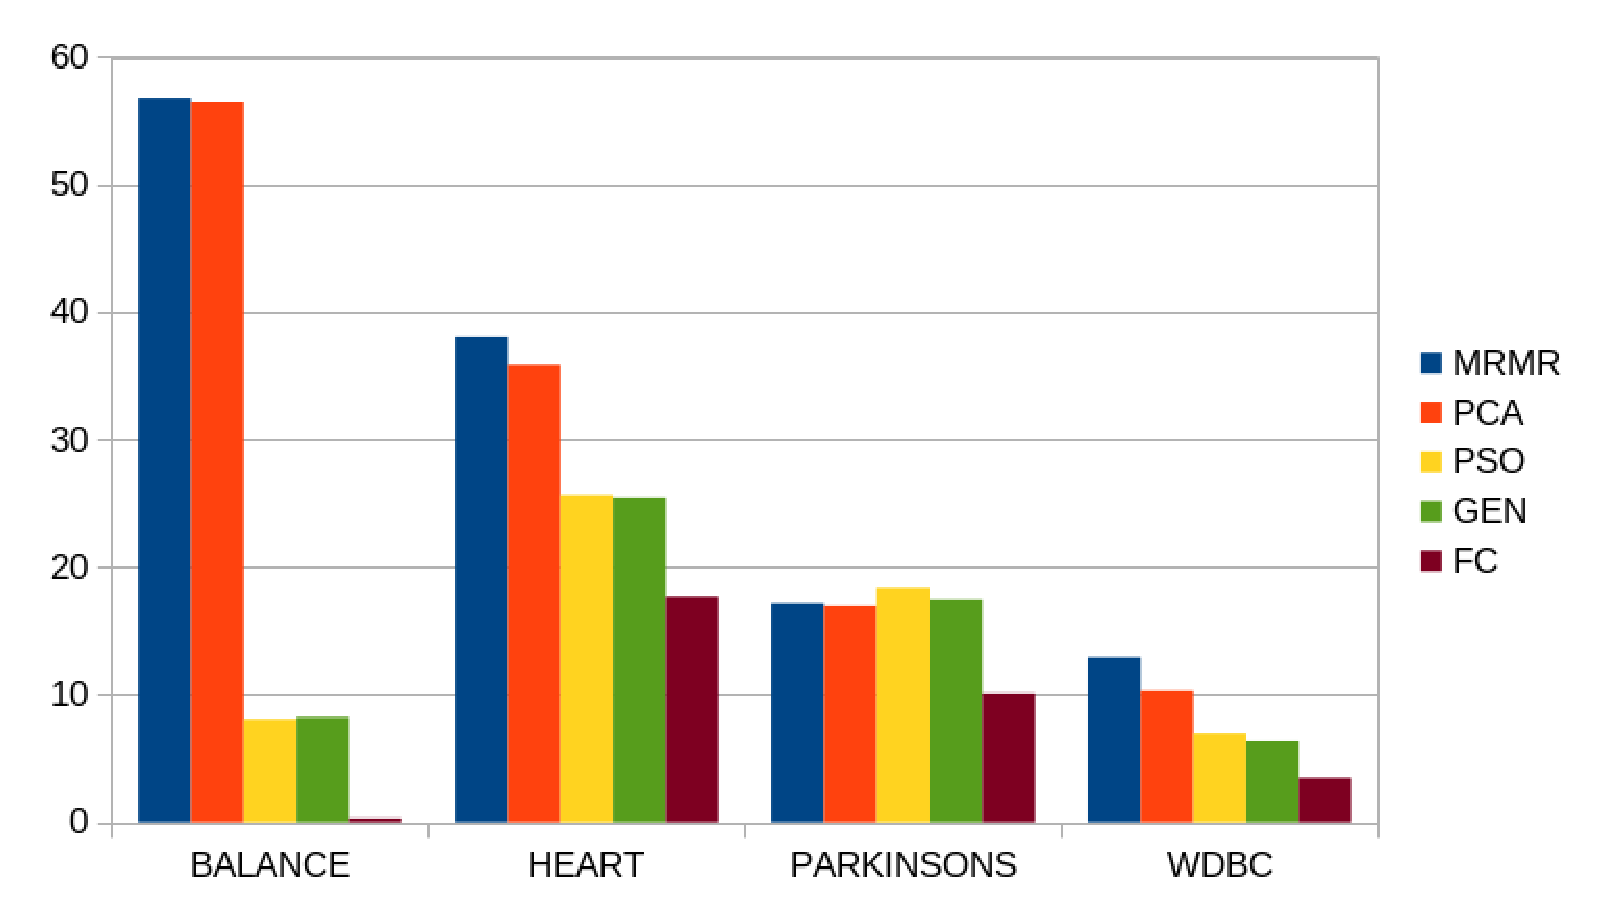
\includegraphics[scale=0.5]{fc_graph_class}
\end{figure}
\begin{table}[H]
\caption{Experiments with the number of chromosomes for the algorithm of subsection
\ref{subsec:Feature-construction}\label{tab:experiments_with_chromosomes}}

\centering{}%
\begin{tabular}{|c|c|c|c|c|}
\hline 
DATASET & $N_{g}=50$ & $N_{g}=100$ & $N_{g}=200$ & $N_{g}=500$\tabularnewline
\hline 
\hline 
HEART & 21.26\% & 21.34\% & 18.73\% & 17.71\%\tabularnewline
\hline 
BK & 0.02 & 0.02 & 0.02 & 0.03\tabularnewline
\hline 
BL & 0.02 & 0.02 & 0.01 & 0.005\tabularnewline
\hline 
FA & 0.01 & 0.01 & 0.01 & 0.01\tabularnewline
\hline 
\end{tabular}
\end{table}


\section{Conclusions\label{sec:Conclusions}}

In the present work, a hybrid feature construction technique was presented
with two phases: a) feature construction and b) feature evaluation.
In the first phase new features were created as non-linear combinations
of old features using Grammatical Evolution and radial base networks.
In the second phase, the original data set was transformed based on
the new features and an artificial neural network with a genetic algorithm
was trained to learn the new data set. The genetic algorithm used
tried to train the artificial neural network in such a way that it
did not lose its generalizing abilities. The proposed technique was
applied to a number of data sets from the relevant literature and
the results were more than satisfactory. Also with a series of additional
experiments the stability of the proposed methodology was shown, since
even with a small number of chromosomes it produces satisfactory results.
However, the proposed technique is much slower than other processes,
as it requires two computational phases to reach a conclusion. However,
with the use of parallel techniques acceleration can be achieved.
The method can be made more efficient in a number of ways, for example
by using parallel genetic algorithms, by using smarter evaluators
to construct features instead of radial base networks such as SVM,
by using more sophisticated termination techniques for genetic algorithm
to achieve acceleration of export of results etc. 
\begin{thebibliography}{10}
\bibitem{nn1}C. Bishop, Neural Networks for Pattern Recognition,
Oxford University Press, 1995.

\bibitem{nn2}G. Cybenko, Approximation by superpositions of a sigmoidal
function, Mathematics of Control Signals and Systems \textbf{2}, pp.
303-314, 1989.

\bibitem{nnphysics1}P. Baldi, K. Cranmer, T. Faucett et al, Parameterized
neural networks for high-energy physics, Eur. Phys. J. C \textbf{76},
2016.

\bibitem{nnphysics2}J. J. Valdas and G. Bonham-Carter, Time dependent
neural network models for detecting changes of state in complex processes:
Applications in earth sciences and astronomy, Neural Networks \textbf{19},
pp. 196-207, 2006

\bibitem{nnphysics3}G. Carleo,M. Troyer, Solving the quantum many-body
problem with artificial neural networks, Science \textbf{355}, pp.
602-606, 2017.

\bibitem{nnchem1}Lin Shen, Jingheng Wu, and Weitao Yang, Multiscale
Quantum Mechanics/Molecular Mechanics Simulations with Neural Networks,
Journal of Chemical Theory and Computation \textbf{12}, pp. 4934-4946,
2016.

\bibitem{nnchem2}Sergei Manzhos, Richard Dawes, Tucker Carrington,
Neural network-based approaches for building high dimensional and
quantum dynamics-friendly potential energy surfaces, Int. J. Quantum
Chem. \textbf{115}, pp. 1012-1020, 2015.

\bibitem{nnchem3}Jennifer N. Wei, David Duvenaud, and Al�n Aspuru-Guzik,
Neural Networks for the Prediction of Organic Chemistry Reactions,
ACS Central Science \textbf{2}, pp. 725-732, 2016.

\bibitem{nnecon1}Lukas Falat and Lucia Pancikova, Quantitative Modelling
in Economics with Advanced Artificial Neural Networks, Procedia Economics
and Finance \textbf{34}, pp. 194-201, 2015.

\bibitem{nnecon2}Mohammad Namazi, Ahmad Shokrolahi, Mohammad Sadeghzadeh
Maharluie, Detecting and ranking cash flow risk factors via artificial
neural networks technique, Journal of Business Research \textbf{69},
pp. 1801-1806, 2016.

\bibitem{nncecon3}G. Tkacz, Neural network forecasting of Canadian
GDP growth, International Journal of Forecasting \textbf{17}, pp.
57-69, 2001.

\bibitem{nnmed1}Igor I. Baskin, David Winkler and Igor V. Tetko,
A renaissance of neural networks in drug discovery, Expert Opinion
on Drug Discovery \textbf{11}, pp. 785-795, 2016.

\bibitem{nnmed2}Ronadl Bartzatt, Prediction of Novel Anti-Ebola Virus
Compounds Utilizing Artificial Neural Network (ANN), Chemistry Faculty
Publications \textbf{49}, pp. 16-34, 2018.

\bibitem{nnc}I.G. Tsoulos, D. Gavrilis, E. Glavas, Neural network
construction and training using grammatical evolution, Neurocomputing
\textbf{72}, pp. 269-277, 2008.

\bibitem{bpnn}D.E. Rumelhart, G.E. Hinton and R.J. Williams, Learning
representations by back-propagating errors, Nature \textbf{323}, pp.
533 - 536 , 1986.

\bibitem{bpnn2}T. Chen and S. Zhong, Privacy-Preserving Backpropagation
Neural Network Learning, IEEE Transactions on Neural Networks \textbf{20},
, pp. 1554-1564, 2009.

\bibitem{rpropnn}M. Riedmiller and H. Braun, A Direct Adaptive Method
for Faster Backpropagation Learning: The RPROP algorithm, Proc. of
the IEEE Intl. Conf. on Neural Networks, San Francisco, CA, pp. 586--591,
1993.

\bibitem{rpropnn3}T. Pajchrowski, K. Zawirski and K. Nowopolski,
Neural Speed Controller Trained Online by Means of Modified RPROP
Algorithm, IEEE Transactions on Industrial Informatics \textbf{11},
pp. 560-568, 2015.

\bibitem{rpropnn2}Rinda Parama Satya Hermanto, Suharjito, Diana,
Ariadi Nugroho, Waiting-Time Estimation in Bank Customer Queues using
RPROP Neural Networks, Procedia Computer Science \textbf{ 135}, pp.
35-42, 2018.

\bibitem{quasinn}B. Robitaille and B. Marcos and M. Veillette and
G. Payre, Modified quasi-Newton methods for training neural networks,
Computers \& Chemical Engineering \textbf{20}, pp. 1133-1140, 1996.

\bibitem{quasinn2}Q. Liu, J. Liu, R. Sang, J. Li, T. Zhang and Q.
Zhang, Fast Neural Network Training on FPGA Using Quasi-Newton Optimization
Method,IEEE Transactions on Very Large Scale Integration (VLSI) Systems
\textbf{26}, pp. 1575-1579, 2018.

\bibitem{psonn}C. Zhang, H. Shao and Y. Li, Particle swarm optimisation
for evolving artificial neural network, IEEE International Conference
on Systems, Man, and Cybernetics, , pp. 2487-2490, 2000.

\bibitem{psonn2}Jianbo Yu, Shijin Wang, Lifeng Xi, Evolving artificial
neural networks using an improved PSO and DPSO \textbf{71}, pp. 1054-1060,
2008.

\bibitem{nndimension}Verleysen M., Francois D., Simon G., Wertz V.,
On the effects of dimensionality on data analysis with neural networks.
In: Mira J., �lvarez J.R. (eds) Artificial Neural Nets Problem Solving
Methods. IWANN 2003. Lecture Notes in Computer Science, vol 2687.
Springer, Berlin, Heidelberg. 2003.

\bibitem{nnpca1}Burcu Erkmen, T�lay Y\i ld\i r\i m, Improving classification
performance of sonar targets by applying general regression neural
network with PCA, Expert Systems with Applications \textbf{35}, pp.
472-475, 2008.

\bibitem{nnpca2}Jing Zhou, Aihuang Guo, Branko Celler, Steven Su,
Fault detection and identification spanning multiple processes by
integrating PCA with neural network, Applied Soft Computing \textbf{14},
pp. 4-11, 2014.

\bibitem{nnpca3}Ravi Kumar G., Nagamani K., Anjan Babu G., A Framework
of Dimensionality Reduction Utilizing PCA for Neural Network Prediction.
In: Borah S., Emilia Balas V., Polkowski Z. (eds) Advances in Data
Science and Management. Lecture Notes on Data Engineering and Communications
Technologies, vol 37. Springer, Singapore. 2020

\bibitem{nngeman}S. Geman, E. Bienenstock and R. Doursat, Neural
networks and the bias/variance dilemma, Neural Computation 4 , pp.
1 - 58, 1992.

\bibitem{nnhawkins}Douglas M. Hawkins, The Problem of Overfitting,
J. Chem. Inf. Comput. Sci. \textbf{44}, pp. 1--12, 2004.

\bibitem{nnsharing1}S.J. Nowlan and G.E. Hinton, Simplifying neural
networks by soft weight sharing, Neural Computation 4, pp. 473-493,
1992.

\bibitem{nnprunning1}S.J. Hanson and L.Y. Pratt, Comparing biases
for minimal network construction with back propagation, In D.S. Touretzky
(Ed.), Advances in Neural Information Processing Systems, Volume 1,
pp. 177-185, San Mateo, CA: Morgan Kaufmann, 1989.

\bibitem{nnprunning2}M.C. Mozer and P. Smolensky, Skeletonization:
a technique for trimming the fat from a network via relevance assesment.
In D.S. Touretzky (Ed.), Advances in Neural Processing Systems, Volume
1, pp. 107-115, San Mateo CA: Morgan Kaufmann, 1989.

\bibitem{nnprunning3}M. Augasta and T. Kathirvalavakumar, Pruning
algorithms of neural networks --- a comparative study, Central European
Journal of Computer Science, 2003.

\bibitem{nndrop1}Nitish Srivastava, G E Hinton, Alex Krizhevsky,
Ilya Sutskever, Ruslan R Salakhutdinov, Dropout: a simple way to prevent
neural networks from overfitting, Journal of Machine Learning Research
\textbf{15}, pp. 1929-1958, 2014.

\bibitem{nnearly1}Lutz Prechelt, Automatic early stopping using cross
validation: quantifying the criteria, Neural Networks \textbf{11},
pp. 761-767, 1998.

\bibitem{nnearly2}X. Wu and J. Liu, A New Early Stopping Algorithm
for Improving Neural Network Generalization, 2009 Second International
Conference on Intelligent Computation Technology and Automation, Changsha,
Hunan, 2009, pp. 15-18.

\bibitem{nndecay1}N. K. Treadgold and T. D. Gedeon, Simulated annealing
and weight decay in adaptive learning: the SARPROP algorithm,IEEE
Transactions on Neural Networks \textbf{9}, pp. 662-668, 1998.

\bibitem{nndecay2}M. Carvalho and T. B. Ludermir, Particle Swarm
Optimization of Feed-Forward Neural Networks with Weight Decay, 2006
Sixth International Conference on Hybrid Intelligent Systems (HIS'06),
Rio de Janeiro, Brazil, 2006, pp. 5-5.

\bibitem{ge1}M. O\textquoteright Neill, C. Ryan, Grammatical evolution,
IEEE Trans. Evol. Comput. \textbf{5,}pp. 349--358, 2001.

\bibitem{fc1}Dimitris Gavrilis, Ioannis G. Tsoulos, Evangelos Dermatas,
Selecting and constructing features using grammatical evolution, Pattern
Recognition Letters \textbf{29},pp. 1358-1365, 2008. 

\bibitem{fc2}Dimitris Gavrilis, Ioannis G. Tsoulos, Evangelos Dermatas,
Neural Recognition and Genetic Features Selection for Robust Detection
of E-Mail Spam, Advances in Artificial Intelligence Volume 3955 of
the series Lecture Notes in Computer Science pp 498-501, 2006.

\bibitem{fc3}George Georgoulas, Dimitris Gavrilis, Ioannis G. Tsoulos,
Chrysostomos Stylios, Jo�o Bernardes, Peter P. Groumpos, Novel approach
for fetal heart rate classification introducing grammatical evolution,
Biomedical Signal Processing and Control \textbf{2},pp. 69-79, 2007 

\bibitem{fc4}Otis Smart, Ioannis G. Tsoulos, Dimitris Gavrilis, George
Georgoulas, Grammatical evolution for features of epileptic oscillations
in clinical intracranial electroencephalograms, Expert Systems with
Applications \textbf{38}, pp. 9991-9999, 2011

\bibitem{genetic1}D. Goldberg, Genetic Algorithms in Search, Optimization
and Machine Learning, Addison-Wesley Publishing Company, Reading,
Massachussets, 1989.

\bibitem{genetic2}Z. Michaelewicz, Genetic Algorithms + Data Structures
= Evolution Programs. Springer - Verlag, Berlin, 1996.

\bibitem{par1}D. J. Doorly , J. Peir�, Supervised Parallel Genetic
Algorithms in Aerodynamic Optimisation, Artificial Neural Nets and
Genetic Algorithms, pp. 229-233, 1997.

\bibitem{par2}Kamal C. Sarma, Hojjat Adeli, Bilevel Parallel Genetic
Algorithms for Optimization of Large Steel Structures, Computer-Aided
Civil and Infrastructure Engineering \textbf{16}, pp. 295-304, 2001.

\bibitem{par3}Yong Fan, Tianzi Jiang, Evans, D.J., Volumetric segmentation
of brain images using parallel genetic algorithms, IEEE Transactions
on Medical Imaging \textbf{21}, pp. 904-909, 2002. 

\bibitem{geneticnn1}F. H. F. Leung, H. K. Lam, S. H. Ling and P.
K. S. Tam, Tuning of the structure and parameters of a neural network
using an improved genetic algorithm, IEEE Transactions on Neural Networks
\textbf{14}, pp. 79-88, 2003.

\bibitem{geneticnn2}A. Sedki, D. Ouazar, E. El Mazoudi, Evolving
neural network using real coded genetic algorithm for daily rainfall--runoff
forecasting, Expert Systems with Applications \textbf{36}, pp. 4523-4527,
2009.

\bibitem{geneticnn3}A. Majdi, M. Beiki, Evolving neural network using
a genetic algorithm for predicting the deformation modulus of rock
masses, International Journal of Rock Mechanics and Mining Sciences
\textbf{47}, pp. 246-253, 2010.

\bibitem{genfc1}M.G. Smith, L. Bull, Genetic Programming with a Genetic
Algorithm for Feature Construction and Selection, Genet Program Evolvable
Mach \textbf{6}, pp. 265--281, 2005.

\bibitem{genfc2}K. Neshatian, M. Zhang, P. Andreae, A Filter Approach
to Multiple Feature Construction for Symbolic Learning Classifiers
Using Genetic Programming, IEEE Transactions on Evolutionary Computation
\textbf{16}, pp. 645-661, 2012.

\bibitem{genfc3}X. Li, M. Yin, Multiobjective Binary Biogeography
Based Optimization for Feature Selection Using Gene Expression Data,
IEEE Transactions on NanoBioscience \textbf{12}, pp. 343-353, 2013.

\bibitem{genfc4}J. Ma, G. Teng, A hybrid multiple feature construction
approach for classification using Genetic Programming, Applied Soft
Computing \textbf{80}, pp. 687-699, 2019.

\bibitem{cover}T.M. Cover, Geometrical and statistical properties
of systems of linear inequalities with applications in pattern recognition,
IEEE Trans. Electron. Comput. EC \textbf{14}, pp. 326--334, 1965.

\bibitem{rbf1}J. Park and I. W. Sandberg, Universal Approximation
Using Radial-Basis-Function Networks, Neural Computation 3, pp. 246-257,
1991.

\bibitem{bnf1}J. W. Backus. The Syntax and Semantics of the Proposed
International Algebraic Language of the Zurich ACM-GAMM Conference.
Proceedings of the International Conference on Information Processing,
UNESCO, 1959, pp.125-132.

\bibitem{tolmin}M.J.D. Powell, A Tolerant Algorithm for Linearly
Constrained Optimization Calculations, Mathematical Programming \textbf{45},
pp 547, 1989.

\bibitem{bfgs2}R. Fletcher, A new approach to variable metric algorithms,
Computer Journal \textbf{13}, pp. 317-322, 1970. 

\bibitem{openmp}R. Chandra, L. Dagum, D. Kohr, D. Maydan,J. McDonald
and R. Menon, Parallel Programming in OpenMP, Morgan Kaufmann Publishers
Inc., 2001.

\bibitem{balance}T. Shultz, D. Mareschal, W. Schmidt, Modeling Cognitive
Development on Balance Scale Phenomena, Machine Learning \textbf{16},
pp. 59-88, 1994.

\bibitem{dermatology}G. Demiroz, H.A. Govenir, N. Ilter, Learning
Differential Diagnosis of Eryhemato-Squamous Diseases using Voting
Feature Intervals, Artificial Intelligence in Medicine. \textbf{13},
pp. 147--165, 1998.

\bibitem{hayesroth}B. Hayes-Roth, B., F. Hayes-Roth. Concept learning
and the recognition and classification of exemplars. Journal of Verbal
Learning and Verbal Behavior \textbf{16}, pp. 321-338, 1977.

\bibitem{heart}I. Kononenko, E. �imec, M. Robnik-�ikonja, Overcoming
the Myopia of Inductive Learning Algorithms with RELIEFF, Applied
Intelligence \textbf{7}, pp. 39--55, 1997.

\bibitem{ion1}J.G. Dy , C.E. Brodley, Feature Selection for Unsupervised
Learning, The Journal of Machine Learning Research \textbf{5}, pp
845--889, 2004.

\bibitem{ion2}S. J. Perantonis, V. Virvilis, Input Feature Extraction
for Multilayered Perceptrons Using Supervised Principal Component
Analysis, Neural Processing Letters \textbf{10}, pp 243--252, 1999.

\bibitem{parkinson}Max A. Little, Patrick E. McSharry, Eric J. Hunter,
Lorraine O. Ramig (2008), 'Suitability of dysphonia measurements for
telemonitoring of Parkinson's disease', IEEE Transactions on Biomedical
Engineering \textbf{56}, pp. 1015-1022, 2009.

\bibitem{popfailures}D.D. Lucas, R. Klein, J. Tannahill, D. Ivanova,
S. Brandon, D. Domyancic, Y. Zhang, Failure analysis of parameter-induced
simulation crashes in climate models, Geoscientific Model Development
\textbf{6}, pp. 1157-1171, 2013.

\bibitem{wine1}M. Raymer, T.E. Doom, L.A. Kuhn, W.F. Punch, Knowledge
discovery in medical and biological datasets using a hybrid Bayes
classifier/evolutionary algorithm. IEEE transactions on systems, man,
and cybernetics. Part B, Cybernetics : a publication of the IEEE Systems,
Man, and Cybernetics Society, \textbf{33} , pp. 802-813, 2003.

\bibitem{wine2}P. Zhong, M. Fukushima, Regularized nonsmooth Newton
method for multi-class support vector machines, Optimization Methods
and Software \textbf{22}, pp. 225-236, 2007.

\bibitem{eeg1}R. G. Andrzejak, K. Lehnertz, F.Mormann, C. Rieke,
P. David, and C. E. Elger, \textquotedblleft Indications of nonlinear
deterministic and finite-dimensional structures in time series of
brain electrical activity: dependence on recording region and brain
state,\textquotedblright{} Physical Review E, vol. 64, no. 6, Article
ID 061907, 8 pages, 2001. 

\bibitem{eeg2}A. T. Tzallas, M. G. Tsipouras, and D. I. Fotiadis,
\textquotedblleft Automatic Seizure Detection Based on Time-Frequency
Analysis and Artificial Neural Networks,\textquotedblright{} Computational
Intelligence and Neuroscience, vol. 2007, Article ID 80510, 13 pages,
2007. doi:10.1155/2007/80510

\bibitem{Stat}J.S. Simonoff, Smooting Methods in Statistics, Springer
- Verlag, 1996.

\bibitem{key23}D. Harrison and D.L. Rubinfeld, Hedonic prices and
the demand for clean ai, J. Environ. Economics \& Management \textbf{5},
pp. 81-102, 1978.

\bibitem{ntdataset}Mackowiak, P.A., Wasserman, S.S., Levine, M.M.,
1992. A critical appraisal of 98.6 degrees f, the upper limit of the
normal body temperature, and other legacies of Carl Reinhold August
Wunderlich. J. Amer. Med. Assoc. 268, 1578--1580

\bibitem{pydataset}R.D. King, S. Muggleton, R. Lewis, M.J.E. Sternberg,
Proc. Nat. Acad. Sci. USA \textbf{89}, pp. 11322--11326, 1992. 

\bibitem{mrmr1}Hanchuan Peng, Fuhui Long, and Chris Ding, Feature
selection based on mutual information: criteria of max-dependency,
max-relevance, and min-redundancy, IEEE Transactions on Pattern Analysis
and Machine Intelligence \textbf{27}, pp.1226-1238, 2005.

\bibitem{mrmr2}Chris Ding, and Hanchuan Peng, Minimum redundancy
feature selection from microarray gene expression data, Journal of
Bioinformatics and Computational Biology \textbf{3}, pp.185-205, 2005

\bibitem{mlpack}Ryan R. Curtin, James R. Cline, N. P. Slagle, William
B. March, Parikshit Ram, Nishant A. Mehta, Alexander G. Gray, MLPACK:
A Scalable C++ Machine Learning Library, Journal of Machine Learning
Research \textbf{14}, pp. 801\textminus 805, 2013. 
\end{thebibliography}

\end{document}
